\documentclass{article}
\usepackage{fullpage}
\usepackage{graphicx}

\title{ExaSAT XML Specification \\ {\large Draft Version 0.3.1}}
\author{Cy Chan \\ ExaCT Co-design Center \\ Lawrence Berkeley National Laboratory}

\begin{document}

\maketitle

This document details the XML file structure used by the ExaSAT (Exascale
Static Analysis Tool).  In typical usage (see Figure~\ref{fig:toolchain}),
the compiler analysis component reads a source code input to generate
an XML file, which is then fed into the performance model component to
estimate imporatant performance statistics (e.g. flops, memory traffic,
working set, runtime).  However, if one wants to estimate the performance
of a hypothetical code formulation without writing the actual code,
an XML representation of that code can be used in conjunction with the
performance model component.

\begin{figure}[ht]
  \begin{center}
    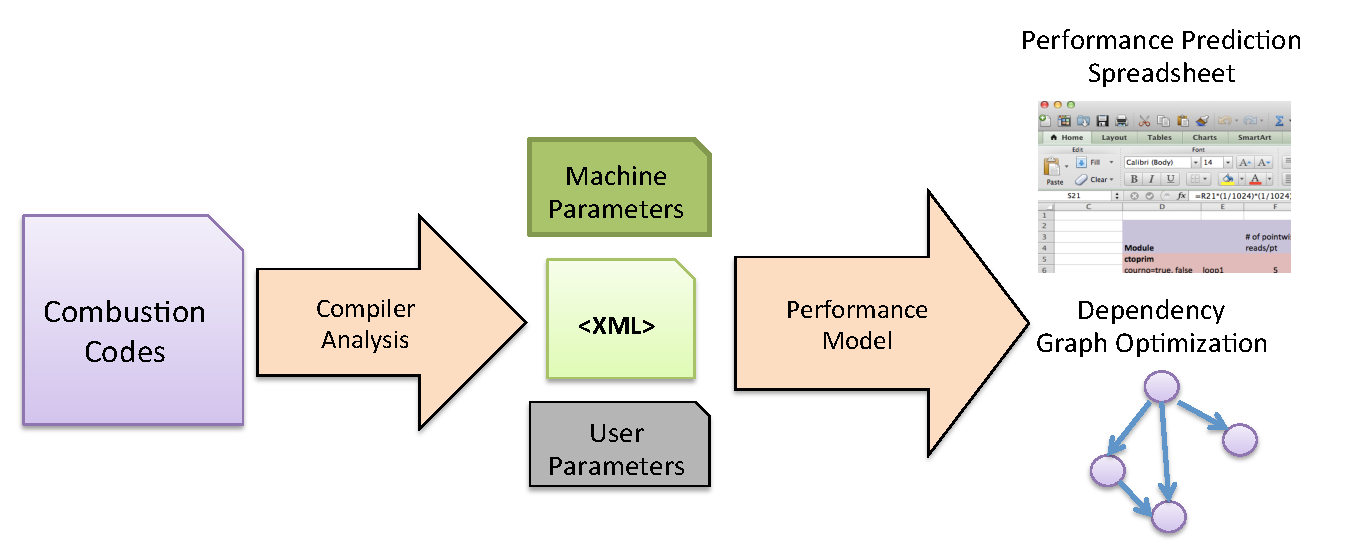
\includegraphics[width=0.7\textwidth]{figs/toolchain}
    \caption{ExaSAT Tool Chain}
    \label{fig:toolchain}
  \end{center}
\end{figure}

\subsection{XML Description}

The XML contains a root {\tt program} element, of which every other
element in the file is a descendant.

\vspace{6mm}
\begin{figure}[ht]
  \begin{center}
    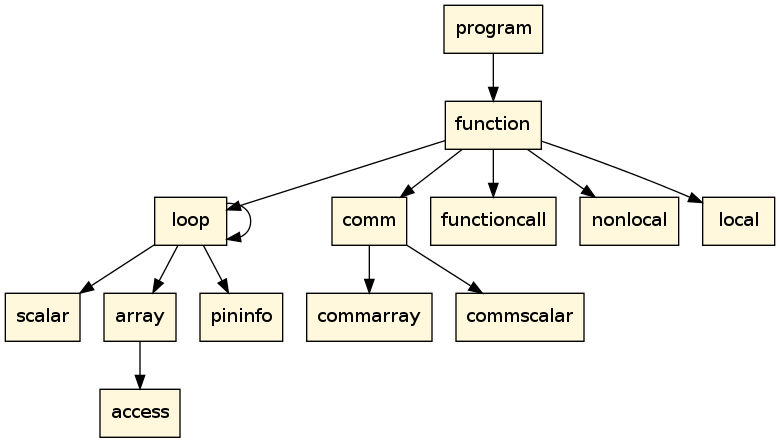
\includegraphics[width=0.7\textwidth]{figs/xml.png}
    \caption{XML Element Hierarchy}
    \label{fig:xml}
  \end{center}
\end{figure}

This section details the attributes and sub-elements found in each
element type.  An element must have exactly one of each attribute listed
for its element type (unless the attribute is designated {\it optional})
and may have zero or more sub-elements of each of the types listed for its
element type.  The elements are presented in the order of a depth-first
traversal of the XML hierarchy as shown in Figure~\ref{fig:xml}.

\subsubsection{The {\tt program} element}
  \begin{itemize}
    \item Attributes: NONE
    \item Sub-Elements:
    \begin{itemize}
      \item {\tt function} - a function that appears in the program
    \end{itemize}
  \end{itemize}

\subsubsection{The {\tt function} element}
  \begin{itemize}
    \item Attributes:
    \begin{itemize}
      \item {\tt name} - the name of the function
    \end{itemize}
    \item Sub-Elements:
    \begin{itemize}
      \item {\tt local} - a local (stack) variable that appears in
        the function
      \item {\tt nonlocal} - a non-local (e.g. global or argument)
        variable that appears in the function
      \item {\tt loop} - a loop that is executed within the function
      \item {\tt comm} - a communication that occurs within the function
      \item {\tt functioncall} - a function call that is made within
        the function
    \end{itemize}
  \end{itemize}

\subsubsection{The {\tt local} element}
  \begin{itemize}
    \item Attributes:
    \begin{itemize}
      \item {\tt name} - the name of the local variable
    \end{itemize}
    \item Sub-Elements: NONE
  \end{itemize}

\subsubsection{The {\tt nonlocal} element}
  \begin{itemize}
    \item Attributes:
    \begin{itemize}
      \item {\tt name} - the name of the non-local variable
    \end{itemize}
    \item Sub-Elements: NONE
  \end{itemize}

\subsubsection{The {\tt loop} element}
  This element is used to help estimate the work needed to execute the
  loop including floating point computation and memory traffic.  Elements
  and attributes associated with a loop pertain to code within that
  particular loop level but not to code further nested in child loops.
  \begin{itemize}
    \item Attributes:
    \begin{itemize}
      \item {\tt linenum} - the line number where the loop begins
      \item {\tt loopvar} - the loop iteration variable
      \item {\tt stride} - the strides used in the loop
      \item {\tt lowerbound} - lower bound of loop
      \item {\tt upperbound} - upper bound of loop
      \item {\tt adds} - the number of floating point additions and
        subtractions in the loop (exclusive of nested child loops)
      \item {\tt multiplies} - the number of floating point
        multiplications in the loop (exclusive of nested child loops)
      \item {\tt divides} - the number of floating point divisions
        in the loop (exclusive of nested child loops)
      \item {\tt specials} - the number of special floating point
        operations (e.g. {\it sqrt}) in the loop (exclusive of nested
        child loops)
    \end{itemize}
    \item Sub-Elements:
    \begin{itemize}
      \item {\tt loop} - a loop nested within this loop
      \item {\tt scalar} - a scalar integer or floating point variable
        that is used in the body of the loop (exclusive of nested
        child loops)
      \item {\tt array} - an integer or floating point array that is
        used in the body of the loop (exclusive of nested child loops)
      \item {\tt pininfo} - a special auxiliary element that is used to
        report performance counter measurements collected during an
        instrumented trial run
    \end{itemize}
  \end{itemize}

\subsubsection{The {\tt scalar} element}
  This element is used to help estimate the number of registers required
  to hold state in the loop body without spilling into the L1 cache.
  It can be used to specify stack variables, global parameters, and
  subroutine arguments.
  \begin{itemize}
    \item Attributes:
    \begin{itemize}
      \item {\tt name} - the name of the scalar variale
      \item {\tt datatype} - the type (e.g. {\tt int} or {\tt double})
        of the variable
      \item {\tt isConstant} - {\tt true} if the variable is a constant
        (e.g. a global or module ``parameter'' in Fortran), or {\tt
        false} otherwise
      \item {\tt reads} - number of reads from the variable during
        the loop (exclusive of nested child loops)
      \item {\tt writes} - number of writes to the variable during
        the loop (exclusive of nested child loops)
    \end{itemize}
    \item Sub-Elements: NONE
  \end{itemize}

\subsubsection{The {\tt array} element}
\label{sec:loopArrayElement}
  This element is used to help estimate the amount of memory traffic
  required to stream data in and out of memory.
  \begin{itemize}
    \item Attributes:
    \begin{itemize}
      \item {\tt name} - the name of the array
      \item {\tt component} - the component of the array (can leave blank)
      \item {\tt datatype} - the type (e.g. {\tt int} or {\tt double})
        of the array
      \item {\tt accesstype} - {\tt readonly, writeonly, readwrite} -
        describes the array access type
      \item {\tt ghost} - the extent of the ghost/halo region accessed
        past the index boundaries, given in the form $((gneg_0, gpos_0),
        (gneg_1, gpos_1), ...)$.  If the index space is $((min_0, max_0),
        (min_1, max_1), ...)$, then the total access space (iteration
        space plus halos) is $((min_0 + gneg_0, max_0 + gpos_0), (min_1 +
        gneg_1, max_1 + gpos_1), ...)$.  Note that by this definition,
        $gneg$ values are typically negative.
    \end{itemize} \item Sub-Elements: \begin{itemize}
      \item {\tt access} - an array access that appears in the loop body
        (exclusive of nested child loops)
    \end{itemize}
  \end{itemize}

\subsubsection{The {\tt access} element}
\label{sec:accessElement}
  This element is used to describe an array location that is accessed in
  the loop.  For relative accesses, the {\tt index} of an access $A(i_0
  + c_0, i_1 + c_1, ..., i_k + c_k)$ is given as a tuple of offsets
  $(c_0, c_1, ..., c_k)$ relative to the loop indices $(i_0, i_1, ...,
  i_k)$, where $k$ is the nesting depth of the loop body, $i_0$ refers
  to the innermost loop variable, and $i_k$ refers to the outermost
  loop variable.  If the loop variables do not appear in the default
  (innermost to outermost) order for that array access, the optional
  {\tt indexorder} attribute is used to specify the order in which the
  loop variables appear.

  TODO: Handle mixed relative and absolute indices.

  \begin{itemize}
    \item Attributes:
    \begin{itemize}
      \item {\tt index} - the index of the access expressed as a tuple
        of offsets relative to the loop indices
      \item {\tt isRelative} - {\tt true} if the index is given relative
        to the loop indices (e.g. {\tt index} $=(0, 1)$ represents $A(i_0,
        i_1 + 1)$), or {\tt false} if the index is fixed (e.g. {\tt index}
        $=(0, 1)$ represents $A(0, 1)$)
      \item {\tt indexorder} ({\it optional}) - a tuple that specifies
        the order in which the loop variables appear in the array access
        tuple.  For example, if {\tt indexorder} is $(0, 2, 1)$, then
        {\tt index} $=(1, 2, 3)$ represents $A(i_0+1, i_2+2, i_1+3)$.
        Defaults to $(0, 1, ..., k)$.
      \item {\tt reads} - number of reads from the array index during
        the loop (exclusive of nested child loops)
      \item {\tt writes} - number of writes to the array index during
        the loop (exclusive of nested child loops)
    \end{itemize}
    \item Sub-Elements: NONE
  \end{itemize}

\subsubsection{The {\tt pininfo} element}
  This special auxiliary element is used to report counters (measured
  by the PINTool dynamic analysis tool), which are collected on a
  per-loop basis during a trial run.  This element differs from most
  other elements in the XML in that it is not used to help describe
  the static structure of the program, but rather to report the code's
  observed behavior during execution.  This information is not currently
  used during performance prediction in the ExaSAT performance model.
  \begin{itemize}
    \item Attributes:
    \begin{itemize}
      \item {\tt entries} - number of entries into the loop
      \item {\tt iters} - number of iterations of the loop
      \item {\tt ops} - total number of all types of operations performed
      \item {\tt reads} - number of read operations
      \item {\tt writes} - number of write operations
      \item {\tt bytereads} - number of bytes read
      \item {\tt bytewrites} - number of bytes written
      \item {\tt uniquereads} - number of unique memory addresses read
      \item {\tt uniquewrites} - number of unique memory addresses written
      \item {\tt adds} - number of additions
      \item {\tt subs} - number of subtractions
      \item {\tt muls} - number of multiplications
      \item {\tt divs} - number of divisions
      \item {\tt cachehits} - number of cache hits
      \item {\tt cachemisses} - number of cache misses
    \end{itemize}
    \item Sub-Elements: NONE
  \end{itemize}

\subsubsection{The {\tt comm} element}
  This element is used to describe communications that occur within
  the function.
  \begin{itemize}
    \item Attributes:
    \begin{itemize}
      \item {\tt linenum} - the line number where the comm begins
      \item {\tt commtype} - the type of communication requested
        (e.g. {\tt reduce} for a reduction or {\tt ghost} for a ghost
        halo exchange)
      \item {\tt interface} - the name of the library function called
    \end{itemize}
    \item Sub-Elements:
    \begin{itemize}
      \item {\tt commscalar} - an integer or floating point variable that
        is communicated
      \item {\tt commarray} - an integer or floating point array that is
        communicated
    \end{itemize}
  \end{itemize}

\subsubsection{The {\tt commscalar} element}
  Currently only used for {\tt commtype="reduce"}.
  \begin{itemize}
    \item Attributes:
    \begin{itemize}
      \item {\tt name} - the name of the variable
      \item {\tt datatype} - the type (e.g. {\tt int} or {\tt double})
        of the variable
    \end{itemize}
    \item Sub-Elements: NONE
  \end{itemize}

\subsubsection{The {\tt commarray} element}
  Currently only used for {\tt commtype="ghost"}.
  \begin{itemize}
    \item Attributes:
    \begin{itemize}
      \item {\tt name} - the name of the array
      \item {\tt datatype} - the type (e.g. {\tt int} or {\tt double})
        of the array
      \item {\tt numofcomponents} - the number of array components
        included in the communication
      \item {\tt ghost} - the extent of the ghost halo region to be
        communicated.  Uses the same format as the {\tt ghost} attribute
        for the {\tt array} subelement of the {\tt loop} element (see
        Section \ref{sec:loopArrayElement}).
    \end{itemize}
    \item Sub-Elements: NONE
  \end{itemize}

\subsubsection{The {\tt functioncall} element}
  \begin{itemize}
    \item Attributes:
    \begin{itemize}
      \item {\tt linenum} - the line number where the function call occurs
      \item {\tt name} - the name of the function call
    \end{itemize}
    \item Sub-Elements: NONE
  \end{itemize}

\subsection{Changelog}

\subsubsection{Changes in Draft Version 0.3.1}

\begin{itemize}
\item added {\tt loopvar} attribute to {\tt loop} element
\item made {\tt reads} and {\tt writes} attributes mandatory for
  {\tt scalar} and {\tt access} elements
\end{itemize}

\subsubsection{Changes in Draft Version 0.3}

\begin{itemize}
\item {\tt loop} elements no longer represent entire loop nests and are
  hierarchically nested to represent each loop statement individually.
  Changed {\tt stride}, removed {\tt range}, and added {\tt lowerbound}
  and {\tt upperbound} to reflect update.  Operation counts and scalar
  and array accesses reflect code in the current loop level only, not
  nested child loops.
\item separated {\tt divides} from {\tt multiplies} attribute in
  {\tt loop} element
\item removed {\tt componentsweep} attribute from {\tt loop} element
\item changed {\tt type} attribute to {\tt datatype} in elements {\tt
  scalar}, {\tt array}, {\tt commscalar}, and {\tt commarray}
\item changed {\tt indextype} attribute to {\tt isRelative}
\item added {\tt cachemisses} attribute to {\tt pininfo} element
\end{itemize}

\subsubsection{Changes in Draft Version 0.2}

\begin{itemize}
\item removed {\tt var} elements, moved children ({\tt local, nonlocal,
  scalar, array}) up one level to {\tt function} or {\tt loop}.
\item removed {\tt flops} element, moved children ({\tt add, multiply,
  special}) up one level to {\tt loop} and changed them to attributes
\item changed loop {\tt range} from element to attribute
\item added {\tt type} attribute to {\tt array} element
\item renamed {\tt access} element's {\tt value} attribute to {\tt index}
\item renamed {\tt access} element's {\tt type} attribute to {\tt
  indextype}
\item added optional {\tt reads} and {\tt writes} attributes to {\tt
  scalar} and {\tt access} elements
\item moved {\tt commtype} attribute into {\tt comm} element
\item renamed {\tt comm} element's {\tt array} sub-element to {\tt
  commarray} for uniqueness
\item added {\tt commscalar} sub-element to {\tt comm} element (for use
  with {\tt commtype="reduce"})
\item added {\tt pininfo} sub-element to {\tt loop} element
\end{itemize}

\end{document}
